\begin{figure*}[t]
\centering
% Preserve the supplied PNG. The two inter-layer labels are corrected in the
% typesetting layer: contenders flow down; certified gain bounds flow up.
\begin{tikzpicture}
\node[anchor=south west,inner sep=0] (figone) at (0,0)
  {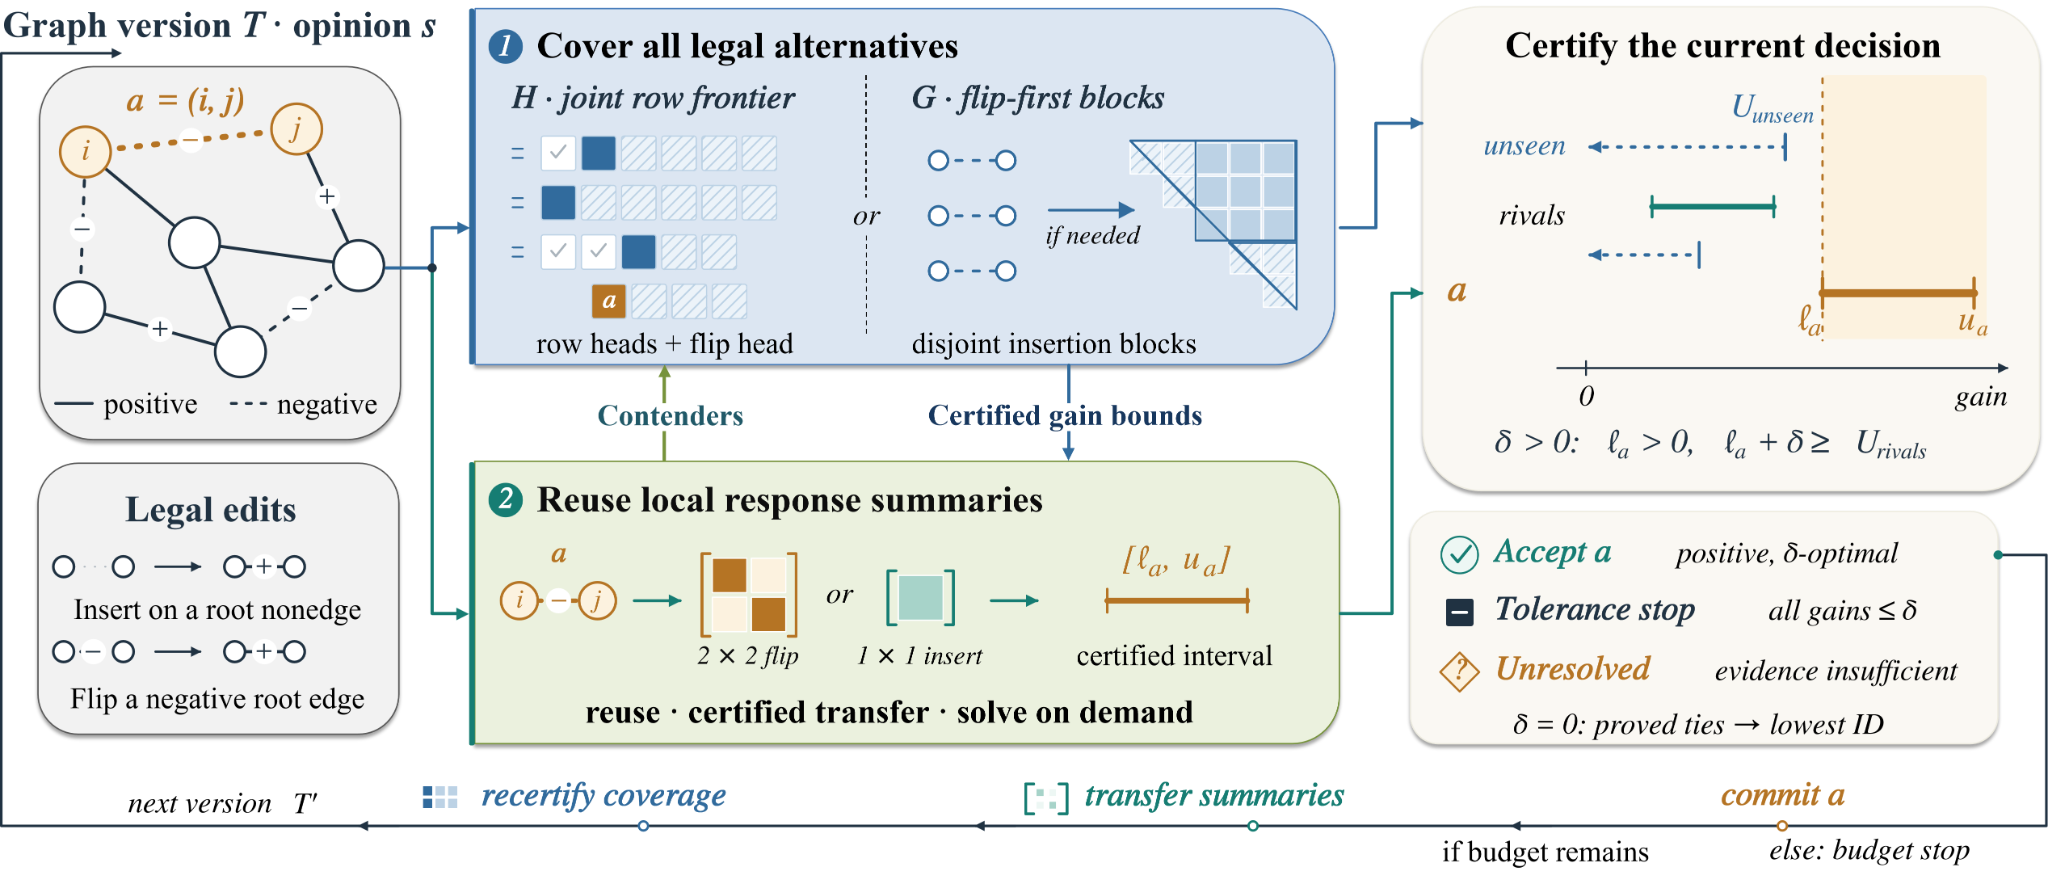
\includegraphics[width=\textwidth]{user_originals/fig1.png}};
\begin{scope}[x={(figone.south east)},y={(figone.north west)}]
\fill[white] (0.2441,0.4994) rectangle (0.6006,0.5420);
\node[font=\bfseries\fontsize{7.2}{8}\selectfont,text=teal!65!black,inner sep=0]
  at (0.3242,0.5207) {Certified gain bounds};
\node[font=\bfseries\fontsize{7.2}{8}\selectfont,text=blue!45!black,inner sep=0]
  at (0.5215,0.5207) {Contenders};
\end{scope}
\end{tikzpicture}
\caption{Current coverage and reusable responses cooperate to certify each edit. H's row frontier or G's block cover identifies contenders; local responses return certified gain bounds. At graph version $T$ with opinion $s$, $[\ell_a,u_a]$ encloses candidate $a$'s gain, $U_{\mathrm{rivals}}$ bounds every other legal candidate, including unseen ones, and $\delta$ is the selection tolerance. An accepted edit advances the version, transfers summaries, and re-establishes coverage while budget remains.}
\Description{A signed graph and its legal edits feed two cooperating layers. Coverage sends contenders to the response layer, which returns certified gain bounds. The current decision combines bounds on unseen candidates and evaluated rivals with a candidate's gain interval. An accepted edit transfers summaries and establishes coverage for the next graph version.}
\label{fig:system}
\end{figure*}
